\documentclass[final]{beamer}
\usepackage{multimedia}
\usepackage{color}
\usepackage[normalem]{ulem}
\graphicspath{{figures/}}

\newcommand{\comment}[1]{}

\mode<beamer>{%
	\usetheme{Madrid}
  \usecolortheme{beaver}
}
\titlegraphic{
\includegraphics[width=0.6\textwidth]{LogoUPF_CBC}}
\title[Italian Academy]{\textbf{The topology of mental states.}\\ Combining data science and graph theory to reveal neural networks for cognitive functions.}
\author{Andrea Insabato}
\institute[]{Universitat Pompeu Fabra \\\vspace{1cm} Italian Academy for Advanced Studies, Columbia University}
\date{November 1st, 2017}

\begin{document}


\begin{frame}<handout:0>
  \titlepage
\end{frame}

\begin{frame}
\transdissolve
\frametitle{The problem}
Characterization of brain networks underlying ``mental'' states 
using data science tools
\pause
\begin{itemize}
	\item mental 
		\pause
	\item brain as a network
		\pause
	\item data science
\end{itemize}
\end{frame}

\begin{frame}
\transdissolve
\frametitle{The problem}
Example: brain network of Alzheimer desease.
\end{frame}

\begin{frame}
\frametitle{The problem: example}
\begin{center}
\includegraphics<2>[width=0.6\columnwidth]{noise_mixture7}
\includegraphics<3>[width=0.6\columnwidth]{noise_mixture6}
\includegraphics<4>[width=0.6\columnwidth]{noise_mixture5}
\includegraphics<5>[width=0.6\columnwidth]{noise_mixture4}
\includegraphics<6>[width=0.6\columnwidth]{noise_mixture3}
\includegraphics<7>[width=0.6\columnwidth]{noise_mixture2}
\includegraphics<8>[width=0.6\columnwidth]{noise_mixture1}
\includegraphics<9>[width=0.6\columnwidth]{noise_mixture0}
\end{center}
\end{frame}

\begin{frame}
\transdissolve
\frametitle{The problem and subproblems}
\begin{itemize}
	\item Characterization of brain networks underlying ``mental'' states 
using data science tools
\pause
	\item Separate different sources of varibility/noise
\pause
	\begin{itemize}
		\item classify individuals
			\pause
		\item classify conditions 
			\pause
		\item extract networks underlying each classification
	\end{itemize}
\end{itemize}
\end{frame}

\begin{frame}
\frametitle{Data}
\begin{itemize}
	\item fMRI
	\item BOLD signal
\end{itemize}
\begin{center}
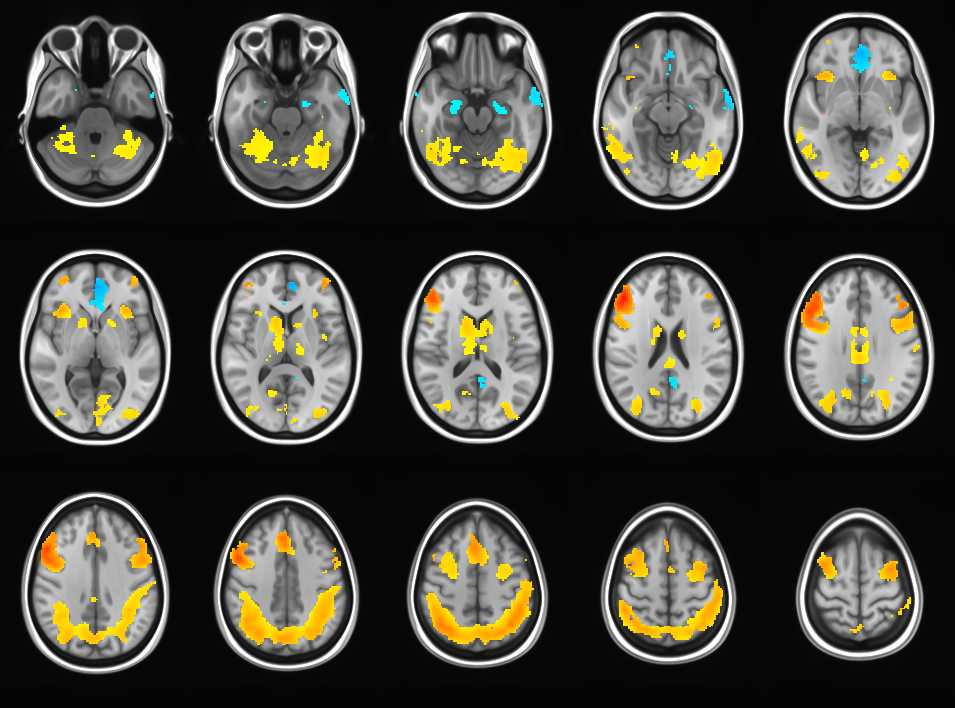
\includegraphics[width=0.7\columnwidth]{fmri}
\end{center}

\end{frame}

\begin{frame}
\frametitle{Data}
\begin{center}
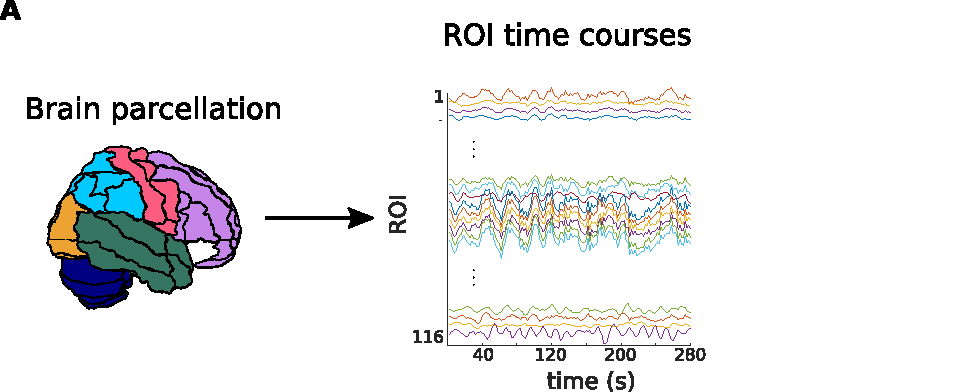
\includegraphics[width=0.8\columnwidth]{fig1b}
\end{center}
\end{frame}

\begin{frame}
\frametitle{Statistical association: correlation}
\begin{center}
\includegraphics<1>[width=0.9\columnwidth]{correlation}
\includegraphics<2>[width=0.5\columnwidth]{toy_FC}
\includegraphics<3>[width=0.8\columnwidth]{correlation_xkcd}
\end{center}
\end{frame}

\begin{frame}
\frametitle{FC}
\begin{center}
\includegraphics<1>[width=0.8\columnwidth]{fig1b}
\includegraphics<2>[width=0.8\columnwidth]{fig1a}
\end{center}
\end{frame}

\begin{frame}
\frametitle{EC}
\begin{center}
\includegraphics<1>[width=0.6\columnwidth]{model}
\transdissolve
\includegraphics<2>[width=0.65\columnwidth]{fitting}
\end{center}
\end{frame}

\begin{frame}
\frametitle{Reduction of ANN to two-equations rate model}
\begin{center}
\includegraphics[width=0.9\columnwidth]{ANN_reduction1}
\end{center}
\vspace{1cm}
\tiny{Wong \& Wang (2006)}
\end{frame}

\begin{frame}
\frametitle{Reduction of ANN to two-equations rate model}
\begin{center}
\includegraphics[width=0.9\columnwidth]{ANN_reduction2}
\end{center}
\vspace{1cm}
\tiny{Wong \& Wang (2006)}
\end{frame}

\begin{frame}
\frametitle{Reduction of ANN to two-equations rate model}
\begin{center}
\includegraphics[width=0.9\columnwidth]{ANN_reduction}
\end{center}
\vspace{1cm}
\tiny{Wong \& Wang (2006)}
\end{frame}

\begin{frame}
\frametitle{confidence in ANN}
\begin{columns}
\begin{column}{0.5\textwidth}
\begin{center}
\includegraphics<1->[width=0.9\columnwidth]{decision_confidence_network_small}
\end{center}
\vspace{1cm}
\tiny{Insabato et al. (2010)}
\end{column}
\begin{column}{0.5\textwidth}
\includegraphics<2>[width=0.9\columnwidth]{confdm_intime_rateraster2}
\end{column}
\end{columns}
\end{frame}

\begin{frame}
\frametitle{Vox populi}
\begin{columns}
\begin{column}{0.5\textwidth}
Galton visits a livestock fair
\begin{center}
\includegraphics<1->[width=0.9\columnwidth]{galton}
\end{center}
\end{column}
\begin{column}{0.5\textwidth}
			\pause
	\begin{itemize}
		\item 800 guesses 
			\pause
		\item mean of the guesses: 1198 pounds
			\pause
		\item weigth of the ox: 1198 pounds
	\end{itemize}
\end{column}
\end{columns}
\end{frame}

\begin{frame}
\frametitle{An ensamble attractor model for decision and confidence}
\pause
\begin{center}
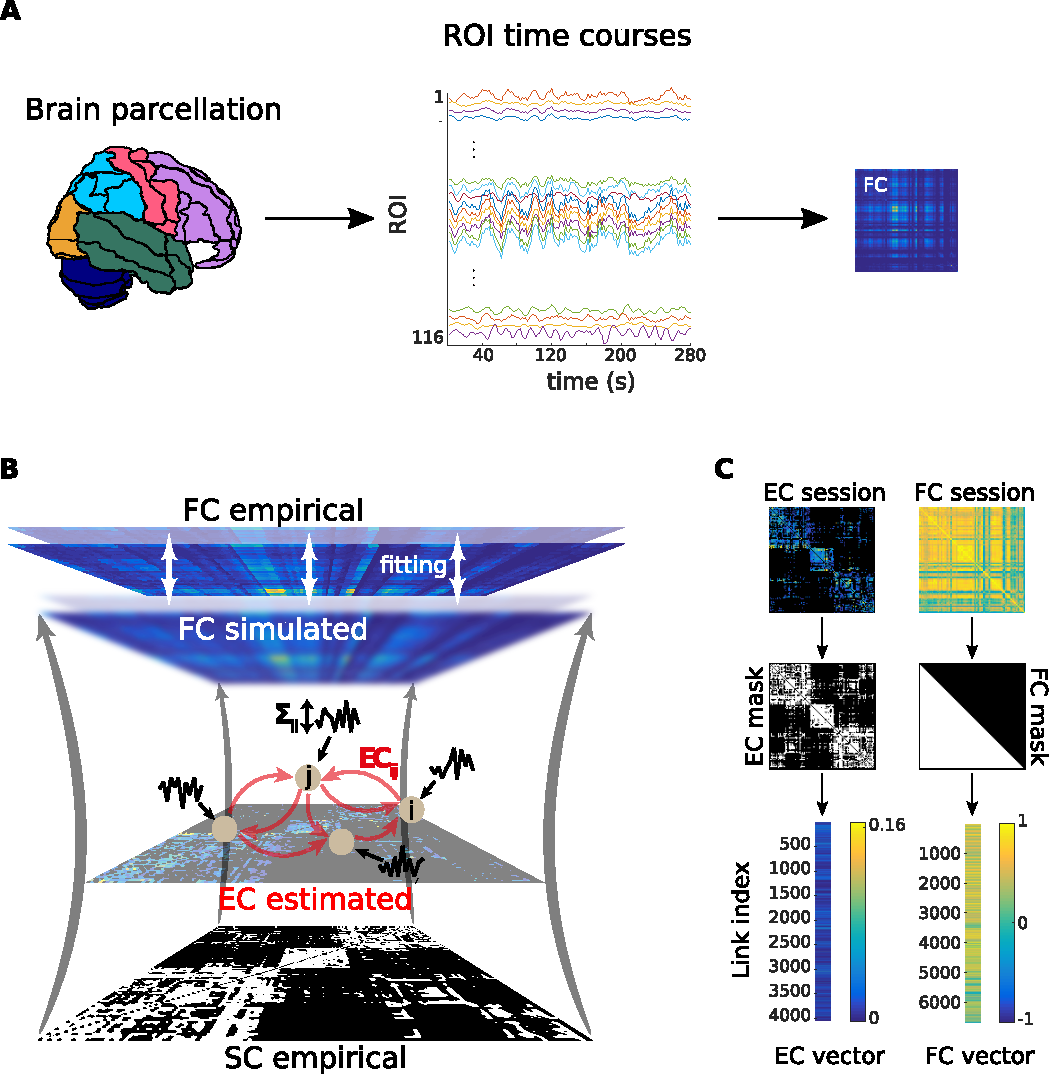
\includegraphics[width=0.9\columnwidth]{fig1}
\end{center}
\vspace{1cm}
\tiny{Paz et al. (2016)}
\end{frame}

\begin{frame}
\frametitle{Dependence of model behavior on IC}
\begin{center}
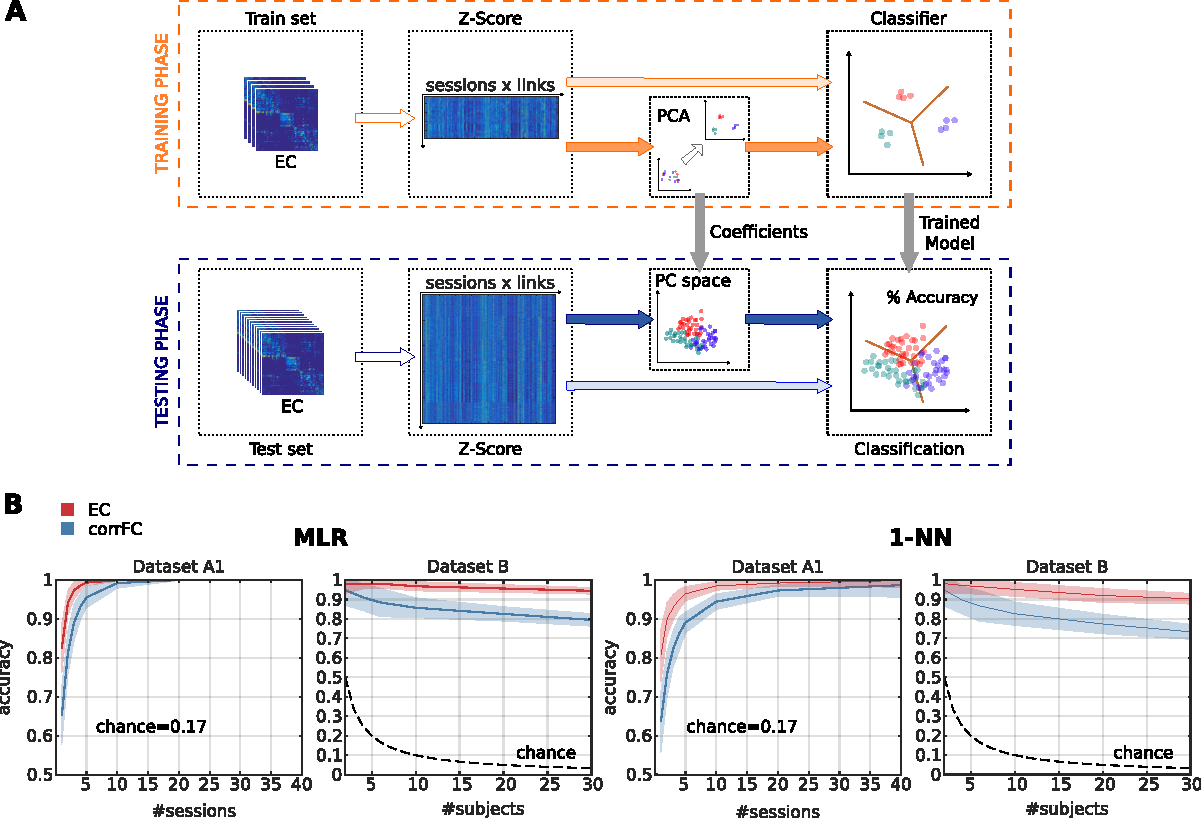
\includegraphics[width=0.8\columnwidth]{fig2}
\end{center}
\vspace{1cm}
\tiny{Paz et al. (2016)}
\end{frame}

\begin{frame}
\frametitle{Estimation of $\sigma_{dv}$}
\pause
\begin{center}
\includegraphics[width=0.8\columnwidth]{fig3_1}
\end{center}
\vspace{1cm}
\tiny{Paz et al. (2016)}
\end{frame}

\begin{frame}
\frametitle{Estimation of $\sigma_{dv}$}
\begin{center}
\includegraphics<1>[width=0.6\columnwidth]{threshold}
\transdissolve
\includegraphics<2>[width=0.8\columnwidth]{full_model}
\end{center}
\vspace{1cm}
\tiny{Lo \& Wang (2006)}
\end{frame}

\begin{frame}
\frametitle{Estimation of $\sigma_{dv}$}
\begin{center}
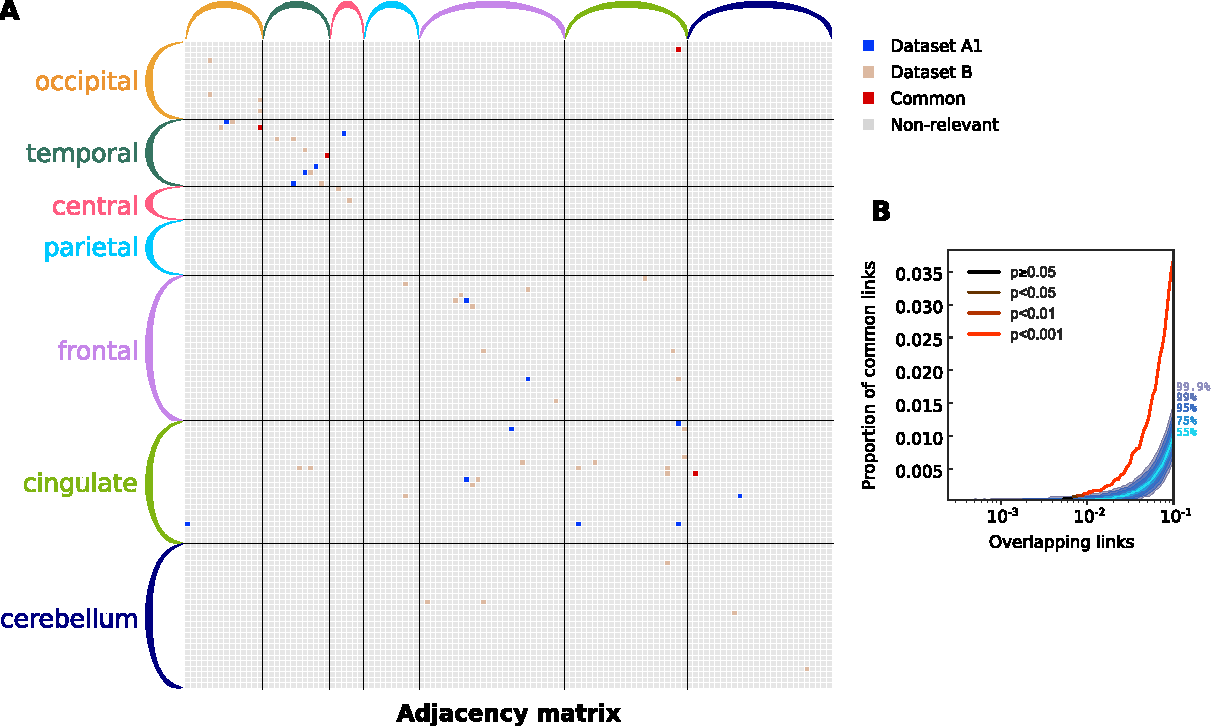
\includegraphics[width=0.8\columnwidth]{fig3}
\end{center}
\vspace{1cm}
\tiny{Paz et al. (2016)}
\end{frame}

\begin{frame}
\frametitle{Fixed duration experiment}
\begin{itemize}
		\pause
	\item Accuracy increases as a function of stimulus duration
		\pause
	\item Confidence increases as a function of stimulus duration 
\end{itemize}
\pause
\begin{center}
\includegraphics[width=0.8\columnwidth]{fixed_duration}
\end{center}
\vspace{1cm}
\tiny{Paz et al. (2016)}
\end{frame}

\begin{frame}
\frametitle{Asymmetric confidence kernels}
\begin{center}
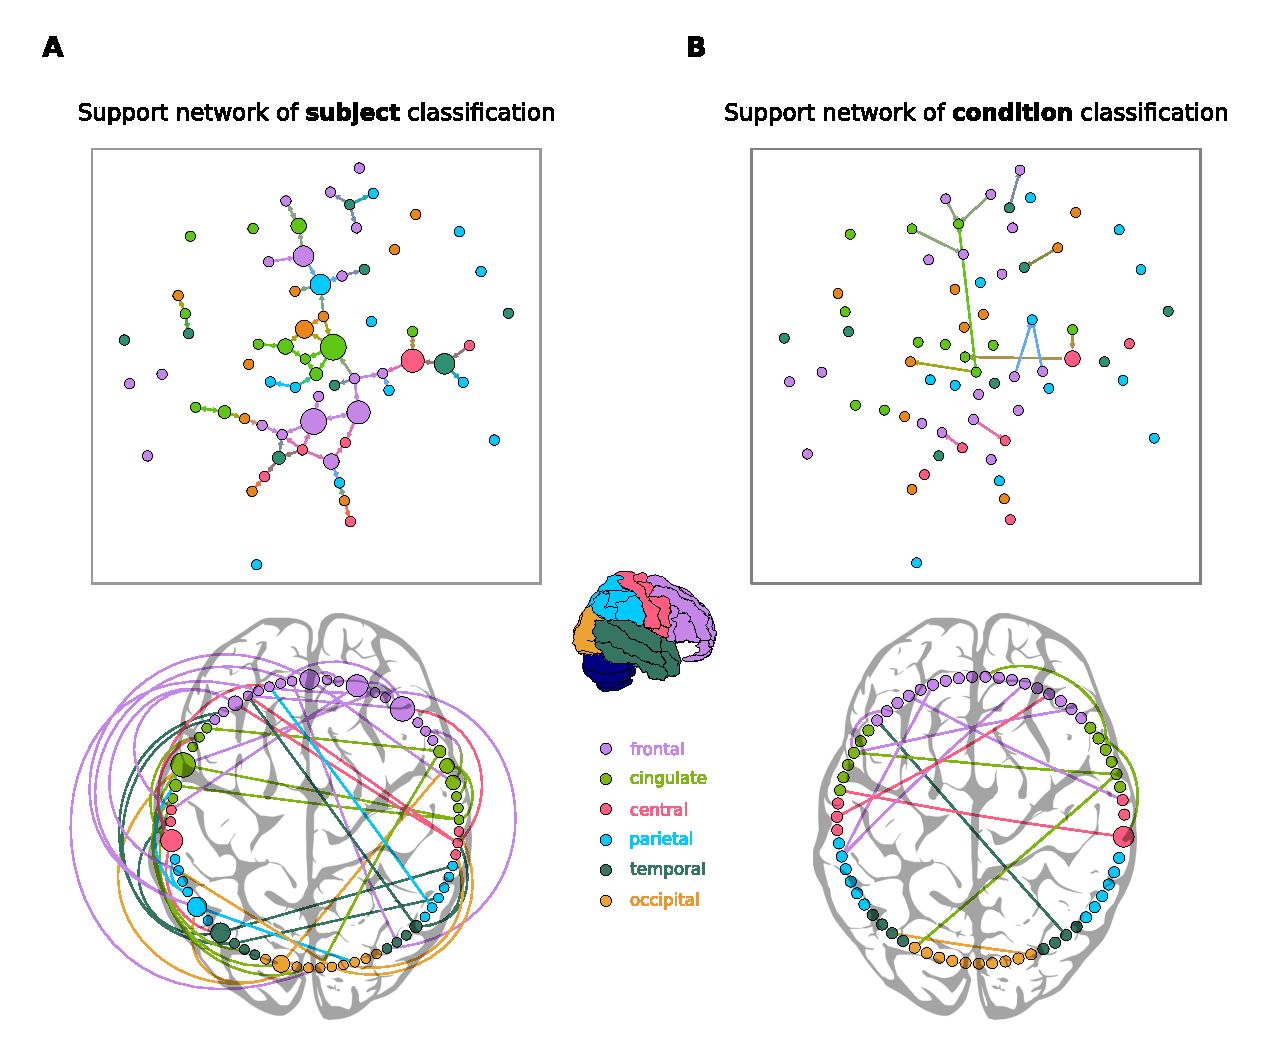
\includegraphics[width=0.6\columnwidth]{fig5}
\end{center}
\vspace{1cm}
\tiny{Paz et al. (2016)}
\end{frame}

\begin{frame}
\frametitle{Asymmetric impact of fluctuations}
\begin{center}
\includegraphics[width=0.8\columnwidth]{fig4}
\end{center}
\vspace{1cm}
\tiny{Paz et al. (2016)}
\end{frame}

\begin{frame}
\frametitle{Reproduction of experimental findings}
\begin{center}
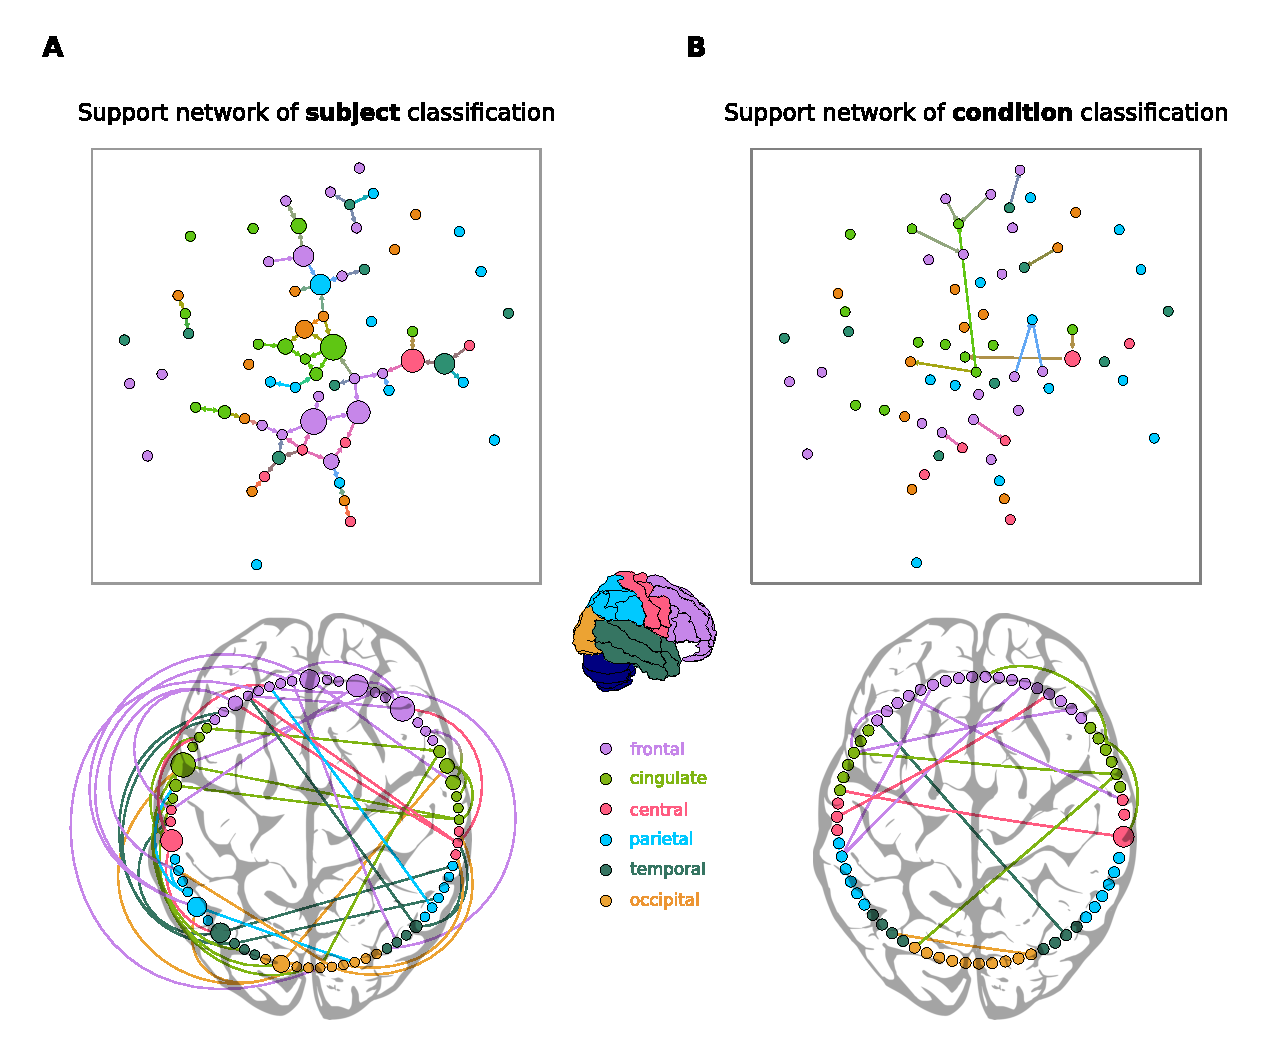
\includegraphics[width=0.9\columnwidth]{fig6}
\end{center}
\vspace{1cm}
\tiny{Paz et al. (2016)}
\end{frame}

\begin{frame}
\frametitle{Summary}
\begin{enumerate}
	\item Confidence can be estimated from the dispersion of modules in an ensamble network
	\item Several experimental findings can be reproduced by this model:
		\begin{itemize}
			\item Confidence is higher for easier stimuli
			\item Confidence decreases as a function of RT 
			\item Choice accuracy and confidence are positively related
			\item Confidence increases as a function of time in fixed duration experiments
			\item Asymmetric confidence kernels
		\end{itemize}
\end{enumerate}
\end{frame}

%\begin{frame}
%\frametitle{}
%\onslide<1>confidence $\rigthwordarrow$ metacognition
%\onslide<2>\color{gray}{(confidence $\rigthwordarrow$ metacognition)}
%\end{frame}

\begin{frame}
\frametitle{Acknowledgments}
\begin{columns}
\begin{column}{0.5\textwidth}
\begin{center}
Luciano Paz\\
\vspace{1cm}

Ariel Zylberberg\\
\vspace{1cm}

Gustavo Deco\\
\vspace{1cm}

Mariano Sigman
\end{center}
\end{column}
\begin{column}{0.5\textwidth}
%\includegraphics[width=0.2\columnwidth,valign=t]{luciano.jpg}
\end{column}
\end{columns}
\end{frame}



\end{document}
